\documentclass[tikz, border=1cm, convert={density=300,outext=.png}]{standalone}
\usetikzlibrary{backgrounds}

\begin{document}

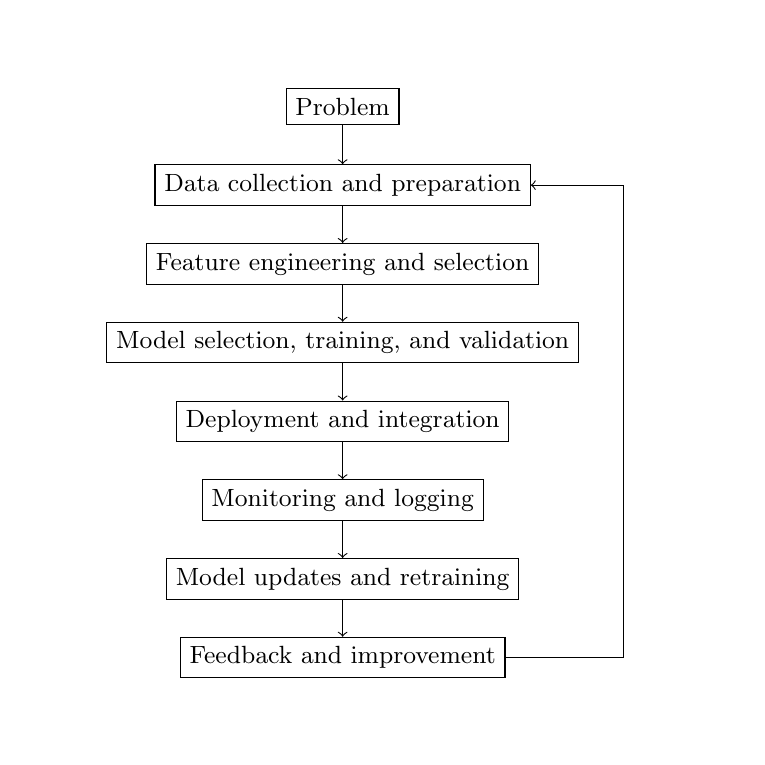
\begin{tikzpicture}[node distance=1cm, every node/.style={font=\small}]
    % white background
    \begin{scope}[on background layer]
        \fill [white] (-4,-8) rectangle (5,1);
    \end{scope}
    % nodes and paths
    \node (problem) [rectangle, draw] {Problem};
    \node (data) [rectangle, draw, below of=problem, align=center] {Data collection and preparation};
    \node (features) [rectangle, draw, below of=data, align=center] {Feature engineering and selection};
    \node (model) [rectangle, draw, below of=features, align=center] {Model selection, training, and validation};
    \node (deploy) [rectangle, draw, below of=model, align=center] {Deployment and integration};
    \node (monitor) [rectangle, draw, below of=deploy, align=center] {Monitoring and logging};
    \node (update) [rectangle, draw, below of=monitor, align=center] {Model updates and retraining};
    \node (feedback) [rectangle, draw, below of=update, align=center] {Feedback and improvement};
    % arrows
    \draw[->] (problem) -- (data);
    \draw[->] (data) -- (features);
    \draw[->] (features) -- (model);
    \draw[->] (model) -- (deploy);
    \draw[->] (deploy) -- (monitor);
    \draw[->] (monitor) -- (update);
    \draw[->] (update) -- (feedback);
    \draw[->] (feedback.east) -| ++(1.5,0) |- (data.east);
\end{tikzpicture}

\end{document}
